\documentclass[tikz, border=1mm]{standalone}

\usetikzlibrary{positioning}

\begin{document}
	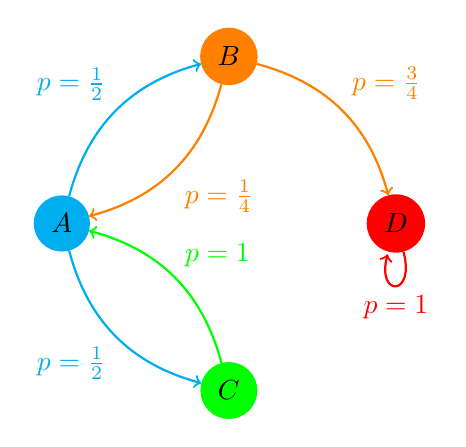
\begin{tikzpicture}[node distance={30mm}, thick, main/.style = {draw, circle, fill}]
		\node[main] (A) [color=cyan] {\textcolor{black}{$A$}};
		\node[main] (B) [above right of=A] [color=orange] {\textcolor{black}{$B$}};
		\node[main] (C) [below right of=A] [color=green] {\textcolor{black}{$C$}};
		\node[main] (D) [below right of=B] [color=red] {\textcolor{black}{$D$}};
		\draw[->, thick, bend left=30, color=cyan] (A) edge node[midway, above left] {$p = \frac{1}{2}$} (B);
		\draw[->, thick, bend right=30, color=cyan] (A) edge node[midway, below left] {$p = \frac{1}{2}$} (C);
		
		\draw[->, thick, bend left=30, color=orange] (B) edge node[midway, above right] {$p = \frac{3}{4}$} (D);
		\draw[->, thick, bend left=30, color=orange] (B) edge node[midway, below right] {$p = \frac{1}{4}$} (A);
		
		\draw[->, thick, bend right=30, color=green] (C) edge node[midway, above right] {$p = 1$} (A);
		
		\path[color=red] (D) edge [anchor=center,loop below] node {$p = 1$} (D);
	\end{tikzpicture}
\end{document}